% \iffalse
\let\negmedspace\undefined
\let\negthickspace\undefined
\documentclass[journal,12pt,twocolumn]{IEEEtran}
\usepackage{cite}
\usepackage{amsmath,amssymb,amsfonts,amsthm}
\usepackage{algorithmic}
\usepackage{graphicx}
\usepackage{textcomp}
\usepackage{xcolor}
\usepackage{txfonts}
\usepackage{listings}
\usepackage{enumitem}
\usepackage{mathtools}
\usepackage{gensymb}
\usepackage{comment}
\usepackage[breaklinks=true]{hyperref}
\usepackage{tkz-euclide} 
\usepackage{listings}
\usepackage{gvv}                                        
\def\inputGnumericTable{}                                 
\usepackage[latin1]{inputenc}                                
\usepackage{color}                                            
\usepackage{array}                                            
\usepackage{longtable}                                       
\usepackage{calc}                                             
\usepackage{multirow}                                         
\usepackage{hhline}                                           
\usepackage{ifthen}                                           
\usepackage{lscape}
\newtheorem{theorem}{Theorem}[section]
\newtheorem{problem}{Problem}
\newtheorem{proposition}{Proposition}[section]
\newtheorem{lemma}{Lemma}[section]
\newtheorem{corollary}[theorem]{Corollary}
\newtheorem{example}{Example}[section]
\newtheorem{definition}[problem]{Definition}
\newcommand{\BEQA}{\begin{eqnarray}}
\newcommand{\EEQA}{\end{eqnarray}}
\newcommand{\define}{\stackrel{\triangle}{=}}
\theoremstyle{remark}
\newtheorem{rem}{Remark}
\begin{document}

\bibliographystyle{IEEEtran}
\vspace{3cm}

\title{GATE: BM - 28.2021}
\author{EE23BTECH11224 - Sri Krishna Prabhas Yadla$^{*}$% <-this % stops a space
}
\maketitle
\newpage
\bigskip

\renewcommand{\thefigure}{\arabic{figure}}
\renewcommand{\thetable}{\arabic{table}}


\vspace{3cm}
\\
\textbf{Results and Derivations:}
\\
Let a function $y\brak{x,t}$ be defined for all $t>0$ and assumed to be bounded. Then we can apply the Laplace transform in t considering x as a parameter.
\begin{align}
 \mathcal{L}\brak{y\brak{x,t}} &= \int_{0}^{\infty}e^{-st}y\brak{x,t}dt\\
 &= Y\brak{x,s}
\end{align}
Let $\frac{\partial y\brak{x,t}}{\partial t}$ be $y_t\brak{x,t}$ and $\frac{\partial y\brak{x,t}}{\partial x}$ be $y_x\brak{x,t}$, then
\begin{align}
 \mathcal{L}\brak{y_t\brak{x,t}} &= \int_{0}^{\infty}e^{-st}y_t\brak{x,t}dt\\
 &= \left. e^{-st}y\brak{x,t}\right|_{a}^{b} + s\int_{0}^{\infty}e^{-st} y\brak{x,t} dt\\
 &= sY\brak{x,s} - y\brak{x,0} \label{L(y_t(x,t))}\\
 \mathcal{L}\brak{y_x\brak{x,t}} &= \int_{0}^{\infty}e^{-st}y_x\brak{x,t}dt\\
 &= \frac{d}{dx}\int_{0}^{\infty}e^{-st}y\brak{x,t}dt \label{L(y_x(x,t))}\\
 &= \frac{dY\brak{x,s}}{dx}
\end{align}

\textbf{Question:} Consider the following first order partial differential equation, also known as the transport equation
\begin{align*}
\frac{\partial y\brak{x,t}}{\partial t}+5\frac{\partial y\brak{x,t}}{\partial x}&=0
\end{align*}
with initial conditions given by $y(x, 0) = \sin x,-\infty < x < \infty$. The value of $y(x, t)$ at $x = \pi$ and $t=\frac{\pi}{6}$ is  \rule{1cm}{0.15mm}.
\begin{enumerate}[label=(\Alph*)]
\item 1
\item 2
\item 0
\item 0.5
\end{enumerate}
\hfill(GATE BM 2021)
\\
\solution
%\fi
\\
From Laplace transforms \eqref{L(y_t(x,t))} and \eqref{L(y_x(x,t))}, we get
\begin{align}
sY(x,s)-y(x,0) + 5\frac{dY\brak{x,s}}{dx} &= 0\\
\implies \frac{dY\brak{x,s}}{dx} + \frac{s}{5}Y\brak{x,s} &= \frac{\sin{x}}{5}
\end{align}
\begin{align}
e^{\frac{s}{5}x}Y\brak{x,s} &= \frac{1}{5} \int e^{\frac{s}{5}x}\sin{x}dx \\
&= \frac{1}{s^2+25}e^{\frac{s}{5}x} \brak{s\sin{x}-5\cos{x}} + c\\
Y\brak{x,s} &= \frac{1}{s^2+25} \brak{s\sin{x}-5\cos{x}} + ce^{-\frac{s}{5}x}
\end{align}
\begin{align}
\label{L(cosat)_BM28} \cos{at} &\system{L} \frac{s}{s^2+a^2} \\
\label{L(sinat)_BM28} \sin{at} &\system{L} \frac{a}{s^2+a^2}
\end{align}
From Laplace transforms \eqref{L(cosat)_BM28} and \eqref{L(sinat)_BM28}, we get
\begin{align}
y(x,t) &= \brak{\brak{\sin{x}\cos{5t}-\cos{x}\sin{5t}}}u(t)+ce^{-\frac{s}{5}x}\delta(t)\\
&= \brak{\sin{\brak{x-5t}}}u(t)+ce^{-\frac{s}{5}x}\delta(t)\\
y(x,0) &= \sin{x}+ce^{-\frac{s}{5}x}\delta(0)\\
\implies c &= 0\\
\therefore y(x,t) &= \brak{\sin{\brak{x-5t}}}u(t)\\
\implies y\brak{\pi,\frac{\pi}{6}} &= 0.5
\end{align}
\begin{figure}[htbp]
	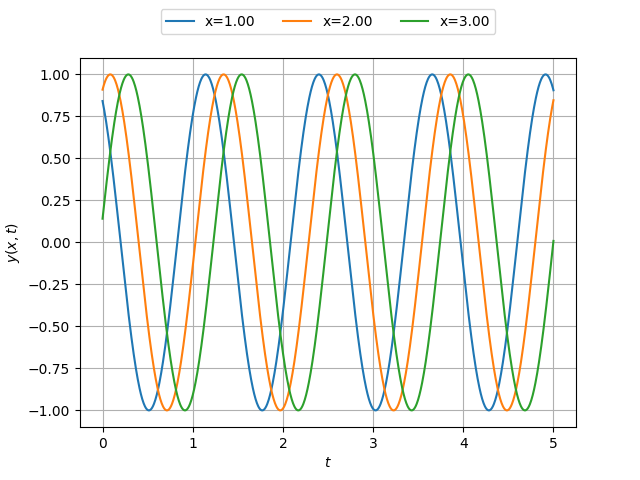
\includegraphics[width=\columnwidth]{figs/plot.png}
	\caption{Plot of $y(x,t)$}
	\label{fig:plot_bm_28}
\end{figure}
\end{document}
